\section{System}
\label{sec:system}

\subsection{Simulation and dock motion}

\begin{figure}[t]
  \centering
  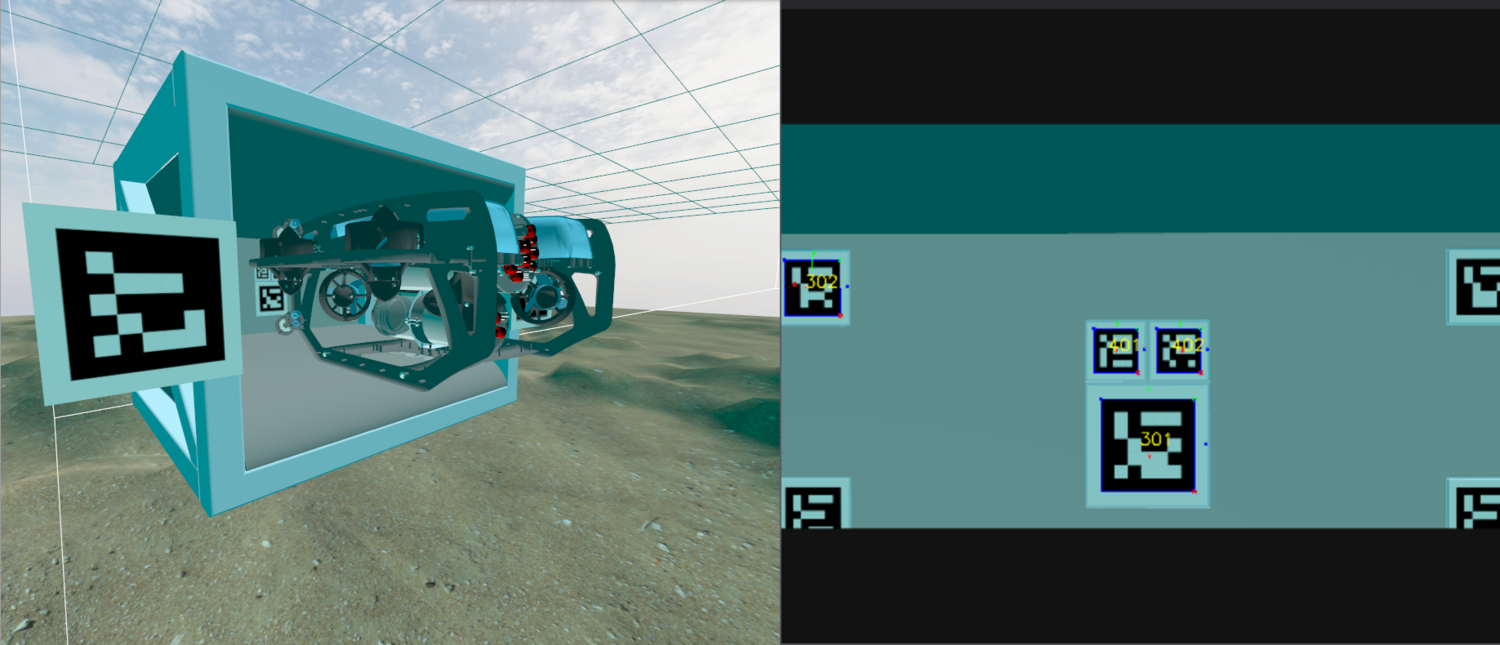
\includegraphics[width=\columnwidth]{figures/sim_views.png}
  \caption{The simulated docking station in Gazebo with the vehicle at the capture envelope (left) and the forward camera's view with the ArUco detections overlaid (right).}
  \label{fig:sim}
\end{figure}

The vehicle is a BlueROV2 Heavy in Gazebo (gz-sim~8, DART physics, Figs.~\ref{fig:sim} and~\ref{fig:arch}) with the production ArduSub firmware executed software-in-the-loop through the ArduPilot Gazebo plugin, so the path from velocity command through mode controller to motor mixing is the code a physical vehicle runs. The vehicle model, hydrodynamics and bring-up derive from the open-source Blue framework \cite{blue2024software,palmer2024angler}, with the drag coefficients aligned to published BlueROV2 Heavy identification. The forward camera renders 1920 by 1080 pixels with a 62$^\circ$ horizontal field of view at 10~Hz, without water-column effects. The world places the docking station 5~m ahead of the spawn point at 1.5~m depth. A plugin drives the dock through a prescribed sinusoidal sway and heave of 0.1~m amplitude with a 90$^\circ$ relative phase, an orbital motion representative of wave forcing on a moored structure, with period and start phase set per trial. Mechanical capture is not modelled; success is defined at the capture envelope and contact with the structure is detected in scoring. The pipeline is the one developed for a static dock in \cite{choi2026thesis}; Table~\ref{tab:params} lists its parameters. The vehicle pose used by every node is the Gazebo ground-truth odometry at 100~Hz, relayed into the transform tree; Section~\ref{sec:failure} depends on this, and Section~\ref{sec:design} replaces it with a corrupted navigation solution.

\begin{figure*}[t]
  \centering
  \scalebox{0.88}{\begin{tikzpicture}[font=\scriptsize, >={Stealth[length=2mm]},
    box/.style={draw, rounded corners=1pt, align=center, minimum height=8mm, inner sep=3pt}]
    \node[box] (cam) {Camera\\(10~Hz)};
    \node[box, right=6mm of cam] (det) {ArUco\\detection};
    \node[box, right=6mm of det] (fus) {Spatial consensus +\\inverse-variance fusion};
    \node[box, right=6mm of fus] (kf) {Error-state\\Kalman filter};
    \node[box, below=10mm of kf] (guid) {Guidance\\(coarse standoff / fine align)};
    \node[box, left=14mm of guid] (ctl) {PBVS control +\\velocity feedforward};
    \node[box, left=14mm of ctl] (veh) {ArduSub\\+ vehicle};
    \node[box, below=8mm of ctl, dashed] (fsm) {Supervisory FSM: \textsc{idle} / \textsc{coarse} / \textsc{fine} / \textsc{docked}};
    \draw[->] (cam) -- (det);
    \draw[->] (det) -- (fus);
    \draw[->] (fus) -- (kf);
    \draw[->] (kf) -- node[right]{\tiny pose, velocity, health} (guid);
    \draw[->] (guid) -- node[above, yshift=1pt]{\tiny error} (ctl);
    \draw[->] (ctl) -- node[above, yshift=1pt]{\tiny cmd\_vel} (veh);
    \draw[dashed, ->] (veh.north) -- node[left]{\tiny camera moves with vehicle} (cam.south);
    \draw[dashed, ->] (fsm.north) -- (ctl.south);
    \draw[dashed, ->] (fsm.east) -| node[right]{\tiny engage / handoff / demote} (guid.south);
  \end{tikzpicture}
}
  \caption{System architecture. The state machine gates the controllers on the filter's health signal; the dashed vehicle-to-camera path is the coupling examined in Section~\ref{sec:failure}.}
  \label{fig:arch}
\end{figure*}

\begin{table}[t]
  \caption{The four arms. All run the world-frame filter live, the same fusion, gates, controllers and state machine.}
  \label{tab:arms}
  \centering
  \footnotesize\setlength{\tabcolsep}{2.5pt}
  \begin{tabular}{@{}>{\raggedright\arraybackslash}p{1.75cm}>{\raggedright\arraybackslash}p{1.35cm}>{\raggedright\arraybackslash}p{1.55cm}>{\raggedright\arraybackslash}p{2.05cm}>{\raggedright\arraybackslash}p{1.35cm}@{}}
    \toprule
    & A reactive & B original & C velocity-closed & D oracle \\
    \midrule
    Process noise & static & sway & sway & sway \\
    Velocity state & pinned at 0 & bounded 0.2~m/s & bounded, decays when stale & bounded 0.2~m/s \\
    Feedforward source & none & $\hat{v}_d$ & $\hat{v}_d$ & true $v_d$ \\
    Feedforward law & -- & open loop, effort & velocity setpoint, PI on $\hat{v}_v$ & open loop, effort \\
    Gain, coarse / fine & -- & 0.6 / 1.0 & $K_p$ 0.30, $K_i$ 0.74 & 0.6 / 1.0 \\
    Position feedback units & effort & effort & m/s (same gains) & effort \\
    \bottomrule
  \end{tabular}
\end{table}

\begin{table}[t]
  \caption{Parameters common to all arms.}
  \label{tab:params}
  \centering
  \footnotesize\setlength{\tabcolsep}{3pt}
  \begin{tabular}{@{}>{\raggedright\arraybackslash}p{1.85cm}>{\raggedright\arraybackslash}p{6.55cm}@{}}
    \toprule
    Markers & 9 ArUco, sides 200, 100 and 47.5~mm; consensus 8$^\circ$, at least 3 agreeing \\
    Measurement noise & $\sigma_p = \alpha r^2/s$, $\alpha = 2.0$ \\
    Filter & 30~Hz predict, $\chi^2$ gate 18.5 (3 dof, 99.9~\%), init on 2 markers \\
    Sway regime & $\sigma_a = 0.16$~m/s$^2$ ($\sqrt{\mathrm{Hz}}$ implied), $|\hat{v}_d| \le 0.2$~m/s \\
    Health & healthy: age $<$ 0.5~s and $\sigma_p <$ 0.02~m; stale: age $>$ 3~s or $\sigma_p >$ 0.15~m \\
    Coarse PD & $K_p$ surge 1.0, sway 0.5, heave 2.0, yaw 1.0; $K_d$ sway 0.3; caps 0.3, 0.3, 0.4~m/s \\
    Standoff and handoff & 1~m out; position 0.10~m, boresight 0.08~m, yaw 0.10~rad, relative speed $<$ 0.15~m/s (EMA 0.3), 10 cycles at 20~Hz \\
    Fine PD & $K_p$ surge 0.4, sway 0.8, heave 2.0, yaw 1.0; $K_d$ surge 0.8, sway 0.3; caps 0.07, 0.15, 0.3~m/s \\
    Align and seat & lateral 0.03, vertical 0.025, yaw 0.05~rad; seat at 0.10~m, 0.03~m, 0.05~rad, 10 cycles \\
    Feedforward & clamp 0.25~m/s; coarse ramp 1.5 to 0.3~m; degraded gain 0.5 \\
    Supervision & 10~Hz; demote after 2~s of loss or 1~s beyond 1.5~m range \\
    Command channel & one unit = full-scale pilot input on the autopilot's manual-control channel \\
    \bottomrule
  \end{tabular}
\end{table}

\subsection{Perception}

The dock face carries nine ArUco markers \cite{garrido2014automatic} in three size classes from 200~mm to 47.5~mm, placed so that the large outer pair carries acquisition at range and the small pair at camera eye level stays in frame during the final centimetres. Each detected marker implies a dock origin through the surveyed layout. A spatial-consensus test on the implied orientations rejects outliers \cite{kim2024enhancing}, and the survivors are fused by inverse-variance weighting \cite{xu2021underwater} with a range-dependent noise model, $\sigma_p = \alpha r^2/s$ for a marker of side $s$ at range $r$, so that distant and small markers count less. The fused pose, in the camera frame, is transformed to the world frame through the vehicle pose at the image stamp and fed to a nine-state error-state Kalman filter over dock position, dock velocity and a small-angle attitude correction. Two process-noise regimes define the two estimators compared throughout: \emph{static}, with zero velocity uncertainty and zero velocity process noise, which is a constant-position filter; and \emph{sway}, with white-acceleration noise of spectral density $\sigma_a^2$ ($\sigma_a = 0.16$~m/s$^2$ nominal), which estimates dock velocity. Each update passes a Mahalanobis gate, the velocity state is bounded at 0.2~m/s, and a health signal reports \textsc{healthy}, \textsc{degraded} or \textsc{stale} from the update age and the position covariance.

\subsection{Guidance, control and supervision}

Guidance converts the filtered dock pose and the vehicle pose into a body-frame error to a target on the dock entry axis, and each phase controller regulates it with position-based visual servoing \cite{chaumette2006visual} (Fig.~\ref{fig:arch}). The coarse controller drives to a standoff point 1~m out along the entry axis with per-axis proportional-derivative gains and a distance-gated surge cap, in the autopilot's depth-hold mode; the handoff to fine alignment is gated on position, boresight offset, yaw and a velocity-match test, debounced so that a sway zero crossing cannot latch it. The fine controller runs align-then-advance in stabilise mode, holding lateral, vertical and yaw tolerances before each step forward, and declares the vehicle seated at a debounced 0.10~m from the entry with 0.03~m lateral and vertical tolerance. A supervisory state machine sequences \textsc{coarse}, \textsc{fine} and \textsc{docked}, demotes on loss of perception, and gates every controller on the filter's health, so a \textsc{stale} estimate produces zero command.

Both controllers accept a dock-velocity feedforward, built from the filter's velocity state rotated into the body frame, clamped at 0.25~m/s and added to the feedback command. The command channel is effort-like: a unit command is full-scale pilot input on the autopilot's manual-control channel, the mode controller maps it to thrust, and the vehicle velocity follows with a gain and a lag. The coarse controller scales the feedforward by a gain of 0.6, ramped in with distance to the standoff, to convert a physical velocity into command units on the basis of a plant gain of 1.3 to 1.6 and a lag of about 240~ms read from a single early trial; the fine controller, which operates at close range, passes it at unit gain, halved while the filter is degraded. In the static regime the velocity state is zero, so the baseline carries no feedforward and the two estimators differ only in the velocity state.
